%Apendice B
%
\chapter{Tablas de carga de la máquina de fatiga}
\label{ch:anexo_b}

\section{Tabla de cargas original}
\label{sec:anexob1}

La siguiente tabla es la que se utiliza actualmente para realizar los ensayos de fatiga en flexión. Se muestra en sus unidades y orden original.

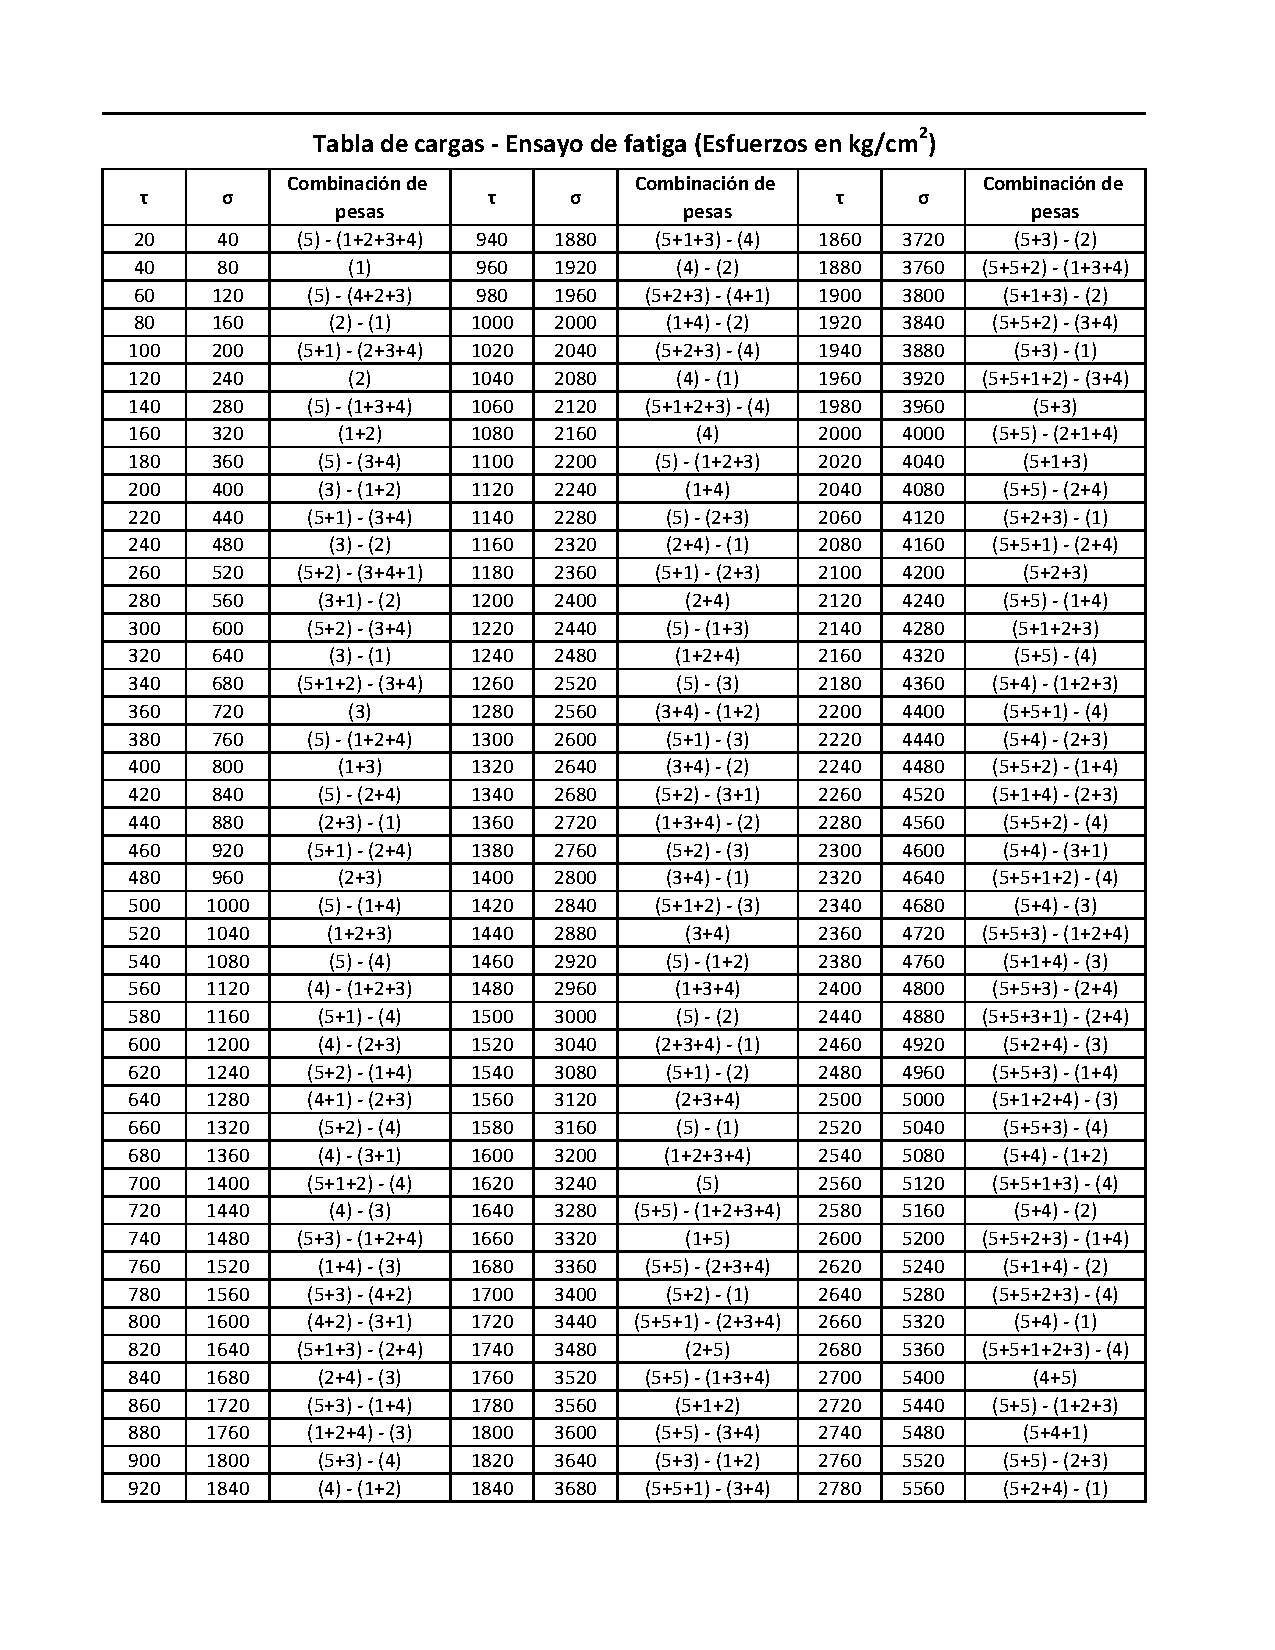
\includepdf[pages=-]{Anexos/anexo_b1.pdf}

\section{Tabla de cargas propuesta}
\label{sec:anexob2}

Esta nueva tabla es la propuesta que emana de los resultados del trabajo realizado. Los esfuerzos de cortante máximo y de von Mises se toman a partir del punto $P$, según la fig. \ref{fig:diag_pqr}. Además, se añade la columna  $F_{max}$ que corresponde a la carga máxima obtenida en el modelo dinámico del sistema para cada combinación de contrapesos.

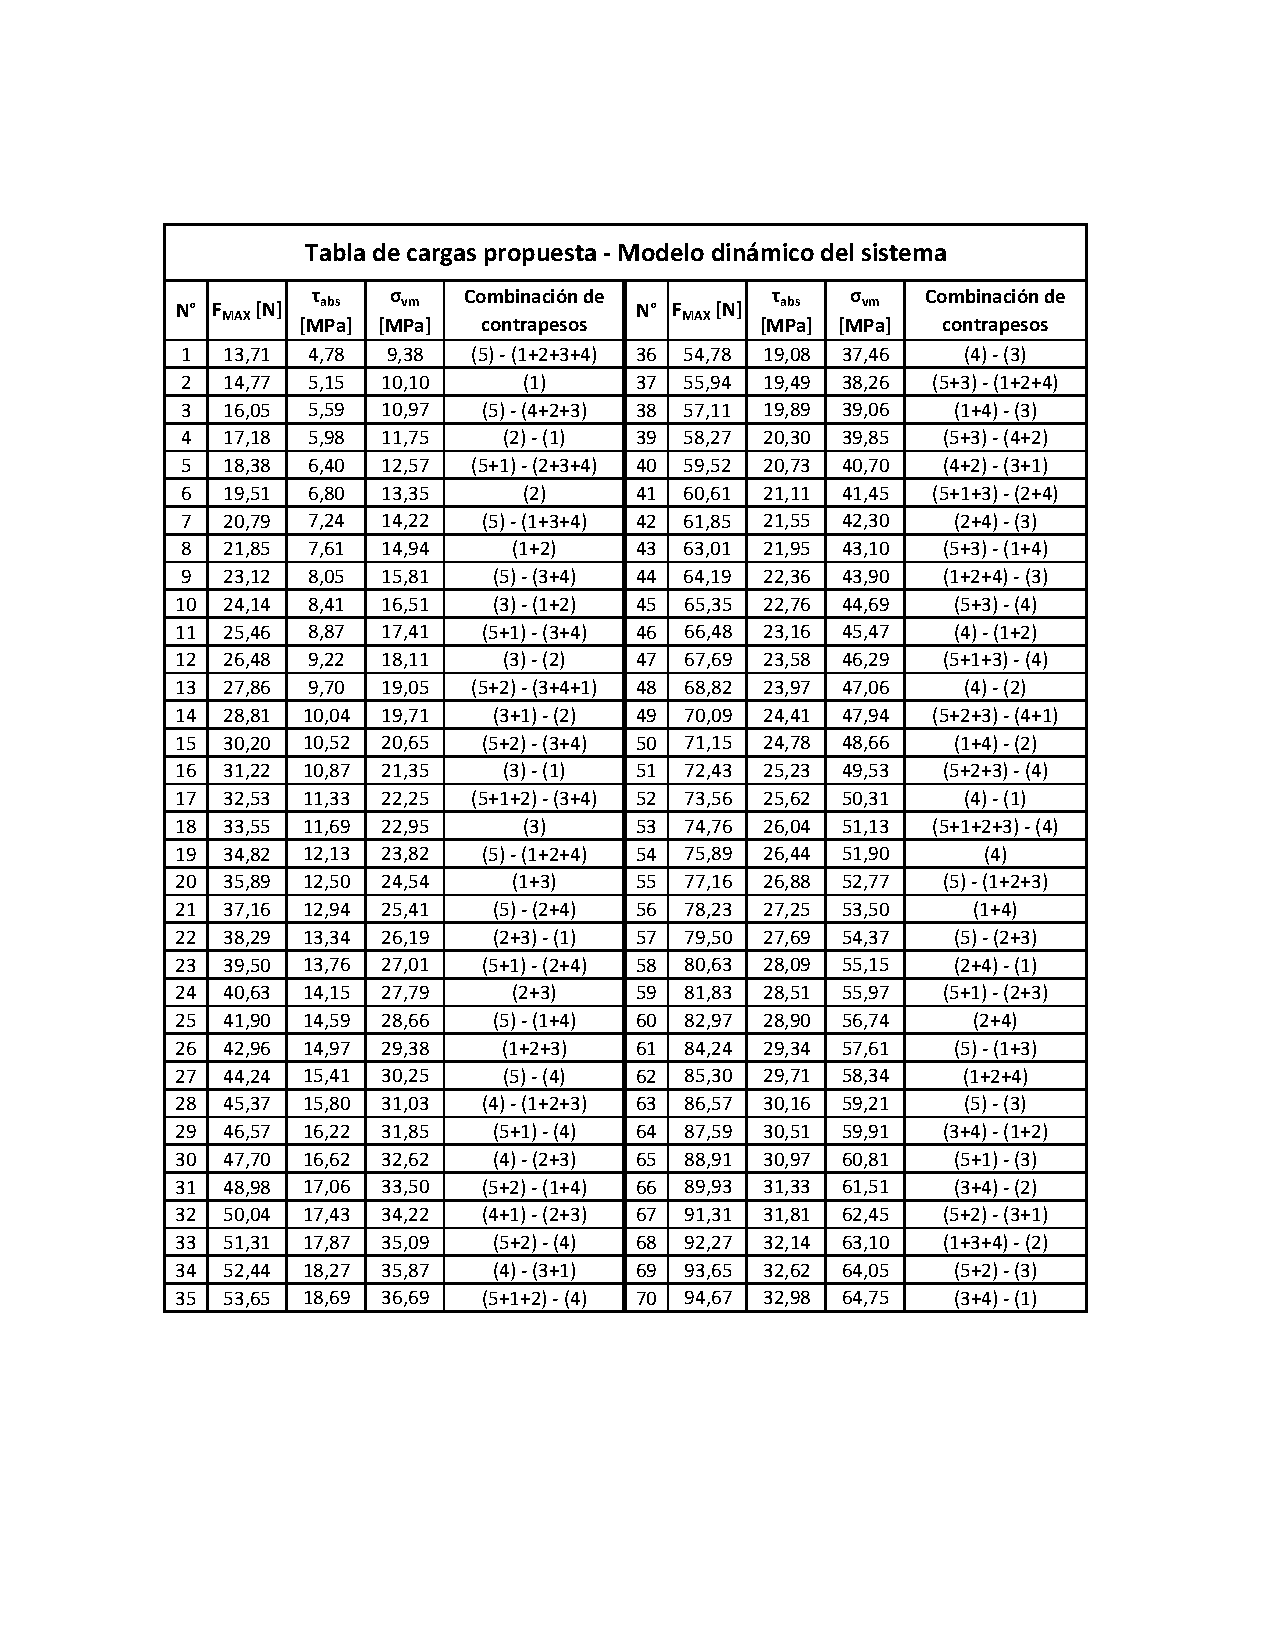
\includepdf[pages=-]{Anexos/anexo_b2.pdf}

\section{Tabla de cargas de la simulación elasto-plástica}
\label{sec:anexob3}

Tabla de las 76 cargas utilizadas para buscar el esfuerzo de fluencia y el esfuerzo último de la probeta. La columna $F_{max}$ corresponde a las cargas aplicadas sobre la probeta. Las columnas $\tau_{max}$ y $\sigma_{vm}$ son los resultados obtenidos para cada nivel de carga. Finalmente, $\Delta m$ es el contrapeso necesario en la máquina para aplicar la carga respectiva, calculada mediante la ec. \ref{eq:deltam}.

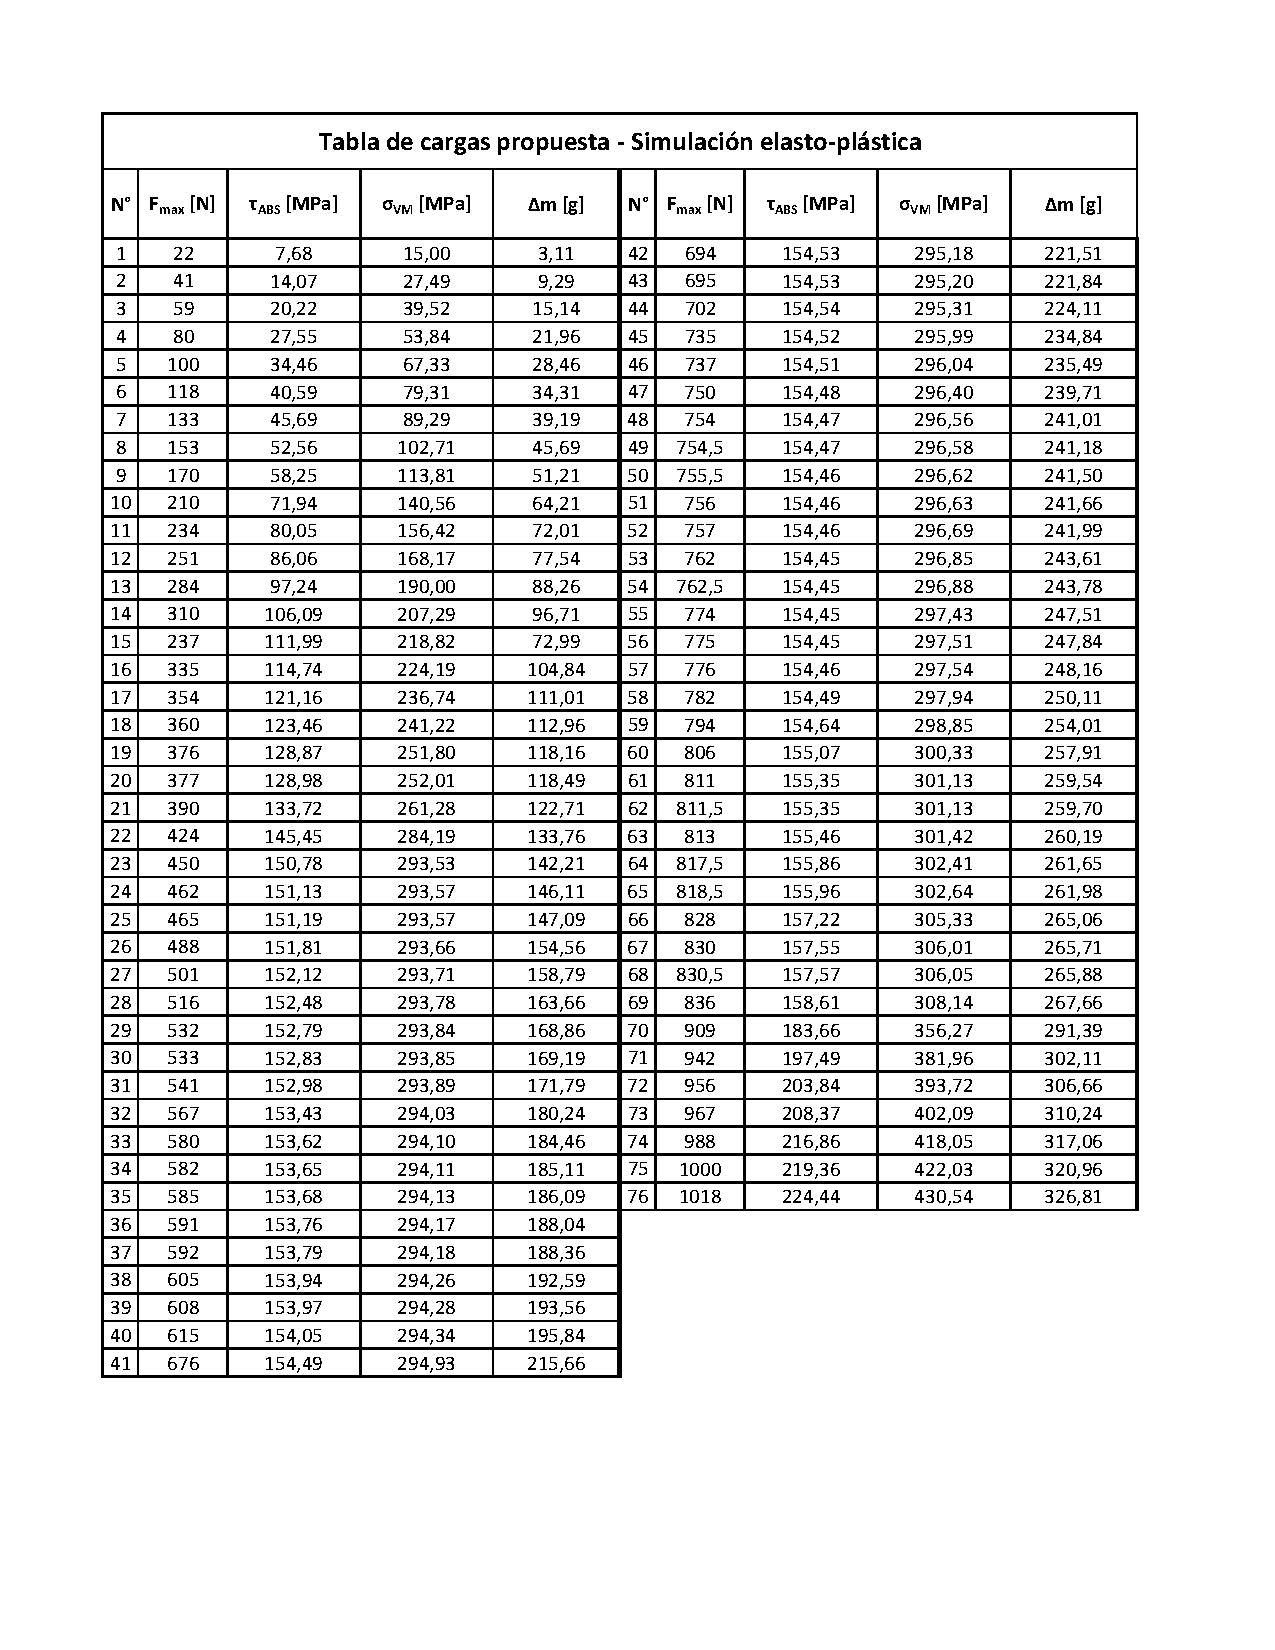
\includepdf[pages=-]{Anexos/anexo_b3.pdf}

\section{Tabla de vida a fatiga esperada}
\label{sec:anexob4}

Tabla de la vida a fatiga esperada para cada carga obtenida mediante el modelo dinámico del sistema. Se muestran los resultados de vida a fatiga obtenidos mediante la relación de Goodman ($N_{f,g}$) y de SWT ($N_{f,swt}$).

